\chapter{Quantum Statistics and Applications}
\label{chapter:quantum_statistics}
%\setcounter{ex}{0}

\section{Introduction}
\label{sec:quantum_statistics_intro}

We have encountered already a number of peculiar features of quantum
mechanics such as wave-particle duality, spatially spread out states,
and point particles with nonzero spin angular momentum.  Now we are
going to add another peculiar feature called \textit{quantum
  indistinguishability} that arises when we make the step up from
one particle to two particles.

What we will see is that quantum particles are indistinguishable in a
way that classical particles cannot be.  And this indistinguishability
has very real consequences, ranging from lasers to superconductors to
white dwarfs.  Most importantly, it is this indistinguishability of
quantum particles that leads to the periodic table and the chemical
properties of the elements, which, needless to say, play a pretty big
role in our everyday existence.


\section{Quantum Statistics}
\label{sec:quantum_statistics_indistinguishability}

The whole phenomenon of indistinguishability results from considering
pairs of quantum particles and asking the following:
\begin{quote}
In a two-particle system where particles 1 and 2 are of the same type,
say, both photons or both electrons, is it possible to tell which is
particle 1 and which is particle 2?
\end{quote}
To be specific, let's consider the ground state of a helium atom.
Helium has two electrons orbiting the nucleus and both electrons can
be in the ground state energy level.  In classical physics, the two
electrons \textit{must} be distinguishable: zoom in with a detailed
enough probe and you could see which electron is where.  You could
name them electron-Fred and electron-George, and then follow their
motion with a fast camera and keep track of which was Fred and which
was George.  So the classical physics answer to the question above is
yes: with enough technology we can tell which is which.

But the microscopic world isn't classical, and in quantum mechanics
things are different.  Heisenberg's uncertainty principle has already
demanded that the electrons in the ground state have some spread in
position and spread in momentum.  Since the two electrons are
overlapping in this smeared out ``Fred-George-blob'' state, Heisenberg
is prohibiting us from tracking the two particles separately, no
matter how fast or high resolution our camera is.  Therefore it is at
least possible for quantum mechanical particles to be
\textit{indistinguishable}.  But that just leaves the question open.
To demonstrate quantum indistinguishability we will have to work out
its implications and then test them against nature.

Let's develop some notation.  If particle 1 is in state
$|\alpha\rangle$ and particle 2 in state $|\beta\rangle$ (these might
be spin states, or energy levels, or whatever), we can write the
two-particle state as $|\psi\rangle = |\alpha\,\beta\rangle$.  Here we
read the particle 1 state as the first symbol and the particle 2 state
as the second symbol.

But if these quantum particles are indistinguishable we cannot really
have the state $|\alpha\,\beta\rangle$, since that notation says we
know it's particle 1 in state $|\alpha\rangle$, and by assumption we
can't know this.  What we really want to say is ``one of the particles
is in $|\alpha\rangle$ and the other particle is in $|\beta\rangle$
and that's all we know.''  We can achieve this by making a
superposition:
\begin{equation}
  |\psi_S\rangle = \frac{1}{\sqrt 2} |\alpha\,\beta\rangle +
  \frac{1}{\sqrt 2}|\beta\,\alpha\rangle.
\end{equation}
The state $|\psi_S\rangle$ truly makes no distinction between particle
1 and particle 2.  You can see this by consider the effect of swapping
the particle labels 1 and 2:
\begin{equation}
  |\alpha\,\beta\rangle 
  \;\xrightarrow[\text{swap } 1\leftrightarrow 2]{} \; 
  |\beta\,\alpha\rangle.
\label{eq:swap_operation}
\end{equation}
If we apply this ``swap'' operation on $|\psi_S\rangle$, we find that
we get the same state back:
\begin{equation}
  |\psi_S\rangle \; \xrightarrow[\text{swap } 1\leftrightarrow 2]{} \;
  \frac{1}{\sqrt 2} |\beta\,\alpha\rangle + \frac{1}{\sqrt 2}
  |\alpha\,\beta\rangle = |\psi_S\rangle.
\end{equation}
Therefore the state $|\psi_S\rangle$, which is the \textit{symmetric}
superposition of $|\alpha\,\beta\rangle$ and $|\beta\,\alpha\rangle$,
is a candidate state to describe indistinguishable
particles.\footnote{The $1/\sqrt{2}$ coefficients are required for
  normalization.}

There is another possibility, though.  Recall that the overall sign of
a wavefunction or state has no impact on any measurable quantity.
All the measurements we can make amount to probabilities, which come
from squaring the coefficients in front of the states.  So we could
also make indistinguishable particle states with the
\textit{antisymmetric} combination
\begin{equation}
 |\psi_A\rangle =  \frac{1}{\sqrt 2} |\alpha\,\beta\rangle
 - \frac{1}{\sqrt 2}|\beta\,\alpha\rangle.
\end{equation}
This state picks up exactly an overall minus sign under the ``swap''
operation:
\begin{equation}
|\psi_A\rangle 
   \;\xrightarrow[\text{swap } 1\leftrightarrow 2]{}  \;
  \frac{1}{\sqrt 2} |\beta\,\alpha\rangle - \frac{1}{\sqrt 2}
 |\alpha\,\beta\rangle
 = -|\psi_A\rangle.
\end{equation}

So we have two possibilities for quantum indistinguishability:
the two-particle states can either be the symmetric $|\psi_S\rangle$
or the antisymmetric $|\psi_A\rangle$.  And now for a strong statement.

\boxittext{Every particle that has ever been
discovered exhibits quantum indistinguishability!}

\noindent This includes photons, electrons, protons, neutrons, the
quarks that make up protons and neutrons, and more exotic particles
like the $W$ and $Z$ bosons.  It seems to be a fundamental property of
the quantum world obeyed by everything, just like wave-particle
duality.

The particles that are symmetric under swap are called
\textit{bosons},\footnote{In honor of the Indian physicist Satyendra
  Bose.} and the particles that are antisymmetric under swap are
called \textit{fermions}.\footnote{In honor of the Italian-American
  physicist Enrico Fermi.}  We will consider both cases in detail
below.


\section{Relation between Statistics and Spin}
\label{sec:statistics_and_spin}

All fundamental particles are either fermions or bosons.  Strangely
enough, which category they fall into is directly determined by their
value of spin.

\begin{itemize}
\item All particles with spin $s=0$, $1$, $2$, \dots or integer spin,
  are bosons: their two-particle states must be symmetric.  This
  includes the photon and some more exotic particles that we will
  encounter in Unit 4.

\item All particles with spin $s=1/2$, $3/2$, etc, which we call
  half-integer spin, are fermions: their two-particle states must be
  antisymmetric.  These include electrons, protons, neutrons, and
  quarks, and more.
\end{itemize}

The connection between the spin of a particle and its symmetry under
exchange (swap) does not have a simple origin, and we will not try to
explain it here.  But it is another rule strictly obeyed by every
particle.

Note that in some cases a collection of particles can act as a single
particle.  For example, a proton is really made up of three quarks.
Each quark is a fermion, so if we imagine exchanging a pair of
protons, we are really exchanging three pairs of quarks.  Each quark
exchange brings in a minus sign, so the net effect of exchanging the
protons in a two-proton state is a factor of $(-1)^3=-1$.  Thus, the proton
will act like a fermion, as long as it makes sense to think of the
proton as a unit, that is, as long as we are not considering some process
that rips apart the protons.

A similar game can be played with entire atoms.  A helium-4 atom
consists of two protons and two neutrons in the nucleus, orbited
by two electrons.  That is an even number of fermions, so if we make a
two-atom state out of two helium atoms, they will be symmetric under
exchange of the atoms.  So the helium-4 atom, if it stays intact, acts
as a boson.

\section{Fermions and the Pauli Exclusion Principle}
\label{sec:~pauli_exclusion_principle}

A very interesting thing happens to fermions in the antisymmetric
two-particle state when the single-particle states $|\alpha\rangle$
and $|\beta\rangle$ are taken to be the same state.  Then we have
\begin{equation}
  |\psi_A\rangle =  \frac{1}{\sqrt 2}|\alpha\, \alpha\rangle - 
  \frac{1}{\sqrt 2}|\alpha\, \alpha\rangle
  = 0.
\end{equation}
What does this mean?  It means that there is no such state!  This is
known as the Pauli exclusion principle, which can be stated as
follows:

\boxittext{\textbf{Pauli exclusion principle:} it is not possible
to put two identical fermions into the same single-particle state.} 

Let's see what it does in practice.  Electrons are fermions.  Consider
an electron in an infinite square-well potential (particle-in-a-box)
% helium atom 
in the lowest energy level $E_1$. 
%This specifies the orbital ($n=1$, $\ell=0$, and $m_\ell=0$), and 
There are
two possible states: $|E_1\hspace{-1mm}\uparrow\rangle$ and
$|E_1\hspace{-1mm}\downarrow\rangle$, meaning ``ground state,
spin up'' and ``ground state, spin down.''

In the ground state, there are two electrons in this lowest
energy level.  If we attempt to put these two electrons in both with
spin up we get
\begin{equation}
  |\psi_A\rangle = \frac{1}{\sqrt 2}|E_1\hspace{-1mm}\uparrow\hspace{2mm} 
  E_1\hspace{-1mm}\uparrow\rangle 
  - \frac{1}{\sqrt 2}|E_1\hspace{-1mm}\uparrow\hspace{2mm} 
  E_1\hspace{-1mm}\uparrow\rangle 
  = 0.
\end{equation}
We find that the state doesn't exist!  The Pauli exclusion principle
tells us we cannot put the two electrons into the ground state with
the spins both up.

But we can put the two electrons into the ground state when their spins
are opposite.  That is, the real ground state is
\begin{equation}
  |\text{He g.s.}\rangle = 
  \frac{1}{\sqrt 2}|E_1\hspace{-1mm}\uparrow\hspace{2mm} 
    E_1\hspace{-1mm}\downarrow\rangle -
  \frac{1}{\sqrt 2}|E_1\hspace{-1mm}\downarrow\hspace{2mm} 
    E_1\hspace{-1mm}\uparrow\rangle.
    \label{eq:helium_ground_state}
\end{equation}
This expression has the proper anti-symmetry and is not zero.

This raises the question of whether we could put three electrons into
the ground state.  As you might guess, there is no three-electron
antisymmetric state $|\psi_A\rangle$, so the upper limit on the number
of electrons we can put into the ground state is two.

\begin{example}{A Five Particle System}
\label{example:five_particles}
Five identical particles with spin $s=1/2$ are put into a
one-dimensional infinite square well with energy levels $E_n=n^2 E_1$
and $E_1=1\units{eV}$.  What is the lowest combined energy that these
particles can have?

\begin{minipage}{3.4in}
%\solution 
\begin{solution}
Two particles can fit into the lowest energy level, in an 
antisymmetric combination like Eq.~(\ref{eq:helium_ground_state}).  Two
more particles can fit into the second lowest energy level, and then one
particle must be in the third energy level.  This is illustrated
schematically on the right.  Adding up these energies:
\[
E_\text{combined} = 1 + 1 + 4 + 4 + 9 = \boxed{19\units{eV}.}
\]
\end{minipage}
\hspace{0.2in}
\begin{minipage}{1.3in}
\includegraphics[width=1.3in]{quantum_statistics/five_particles}
\end{minipage}

\end{solution}
\end{example}

Pauli's Exclusion Principle has {\bf tremendously} important implications
for the behavior of atoms and for the entire field of chemistry (and,
therefore, biology as well). We'll discuss these implications in the
next chapter.

\section{Bosons}
\label{sec:bosons}

Now let's turn to bosons, the particles that form symmetric
combinations $|\psi_S\rangle$ in their two-particle states.  These
particles do not exhibit a Pauli exclusion principle.  In fact, it's
quite the opposite: bosons like to be in the same state, relative to
distinguishable particles.\footnote{Okay, no one has actually managed
  to interview a boson to confirm their feelings on the matter, but we
  can observe their behavior and draw some conclusions.}

Demonstrating this effect is a little bit tricky.  Let us consider the
following scenario: imagine that there are three different states,
which we'll call $|\alpha\rangle$, $|\beta\rangle$, and
$|\gamma\rangle$, and there are two particles which will be put into
those states.  How many possible two-particle states are there?

For classical distinguishable particles, each particle can be in one
of three possible states, so there are $3\times 3=9$ possible
two-particle states.  These are illustrated in the chart on the left
in Fig.~\ref{fig:quantum_statistics}.  Since the particles are
distinguishable, we use different symbols for them: ``$\bullet$''
for particle 1 and ``$\circ$'' for particle 2.

\begin{figure}[h]
\begin{center}
\includegraphics[width=4.8in]{quantum_statistics/quantum_statistics_table}
\caption{The distinguishable classical particles are indicated by a
  filled circle $\bullet$ and an empty circle $\circ$.  The
  indistinguishable quantum particles are both indicated by a filled
  circle.}
\label{fig:quantum_statistics}
\end{center}
\end{figure}

Now consider indistinguishable bosons, shown in the middle chart of
Fig.~\ref{fig:quantum_statistics}.  Now any two states that differ by
an exchange of particles only gets counted once.  For example, the
classical case of having the $\bullet$ particle in state $\alpha$ and
the $\circ$ particle in state $\beta$ (row 4) is different from the
case where the two particles are switched (row 7).  But for
indistinguishable bosons these are the same state, so it only appears
once (row 4 for the bosons).

Finally, for fermions it is pretty straightforward.  They are
indistinguishable, so we just use $\bullet$ for both particles, and we
add in the Pauli exclusion principle, which eliminates the cases where
both particles are in the same state.  This gives the chart on the
right in Fig.~\ref{fig:quantum_statistics}.

What do we learn from these charts?  Let's consider the case where the
three states, $|\alpha\rangle$, $|\beta\rangle$, and $|\gamma\rangle$,
all have the same energy.  If these quantum states are in thermal
equilibrium, we can appeal to ergodicity to argue that every
two-particle microstate is equally probable.  And this gives us
something interesting.

Look at the probability of finding two particles in the same state.
For the distinguishable classical particles, there are 3 cases out of
9 where the particles are in the same state, so it's a probability of
$1/3$.  But for the bosons, there are 3 cases of out 6 where they are
in the same state, so a probability of $1/2$.  Indistinguishability
has given the bosons an \textit{enhanced} probability of being in the
same state.  It is almost as if the bosons have an attractive force
pulling them into the same state, but really it's just a property of
their statistics.

And this turns out to have quite an impact.  When there are a large
number of identical bosons in a system, the statistical ``attraction''
becomes even more powerful and it is sometimes possible to get a
macroscopic fraction of the particles to cram together into the same
quantum state.  This state is called then a Bose condensate.  When we
achieve this, we end up with a material that exhibits quantum
mechanical properties on our everyday macroscopic scale, which is
truly bizarre.

We have managed to make Bose condensates with a number of different
types of bosons.  When we do this with photons, we get a laser.  When we
do this with helium-4 atoms, we get a superfluid.  When we do this with
electrons paired up to be bosons (more below), we get a superconductor.
Most recently, physicists have figured out how to get a gas of large atoms,
such as rubidium, to form a Bose-Einstein condensate.  These are all very
different systems with very different properties, and we devote the remainder
of the chapter to describing some of them.

\section{Lasers}
\label{sec:lasers}

The word ``laser'' is an acronym for \textbf{L}ight
\textbf{A}mplification by \textbf{S}timulated \textbf{E}mission of
\textbf{R}adiation.  Einstein predicted the essential process of
\textit{stimulated emission} (described below) based on his analysis
of how light interacts with atoms, but it took nearly a half-century
until we were able to construct an operating laser. Now lasers appear
in dozens of commercial products including supermarket scanners and
blue-ray disc players. They are also used for cutting and shaping in
manufacturing, as scalpels in delicate eye surgery, and as tools in
countless scientific experiments.

\begin{figure}[t]
\begin{center}
\includegraphics[width=4.8in]{quantum_statistics/photon_process}
\caption{Three processes in which photons interact with a two-level
  atom.}
\label{fig:photon_process}
\end{center}
\end{figure}

So just what is stimulated emission?  Consider a pair of energy levels
for an electron in an atom, as shown in Fig.~\ref{fig:photon_process},
with energy difference $\Delta E$.  These need not be neighboring
energy levels.  We have learned already about the processes of
absorption and spontaneous emission, which are shown in parts (a) and
(b) of Fig.~\ref{fig:photon_process}.  Recall that the absorbed or
emitted photon must have energy $E_\text{ph}=\Delta E$ due to energy
conservation.  


Einstein realized\footnote{Einstein used some
  interesting thermodynamics arguments to discover stimulated
  emission.  You can learn about these in PHYS 222.}  there must also
be a third process of stimulated emission, which involves an incoming
photon of energy $E_\text{ph} = \Delta E$ and an electron in the upper
energy level (see Fig.~\ref{fig:photon_process}c).  This appears to be
an unlikely candidate for a photon-electron interaction, since the
electron is already in the upper energy level.  But photons have spin
$s=1$, which makes them bosons, and that means photons are
``attracted'' to be in the same state.  The incoming photon induces
the electron to jump down to the lower energy level and emit a second
photon with the same energy, in essence ``cloning'' itself.  In fact,
this second photon is in exactly the same quantum state as the
incoming photon.  This means, among other things, that they have the
same momentum vector, and so they are traveling in the same direction.


\begin{figure}
\begin{center}
\includegraphics[width=4.4in]{quantum_statistics/laser_cavity}
\caption{Schematic drawing of a gas laser showing laser cavity
  containing atoms and radiation (photons). Empty circles $\circ$ are
  atoms in the lower energy states and filled circles $\bullet$ are
  atoms in a higher energy state.}
\label{fig:laser_cavity}
\end{center}
\end{figure}

So how do we make a laser from this?  The very first lasers consisted
of a gas of atoms contained within a resonant cavity composed of a
glass tube sealed at either end with mirrors, as shown in
Fig.~\ref{fig:laser_cavity}.  These atoms are chosen to have a
suitable pair of energy levels, $E_\text{upper}$ and $E_\text{lower}$,
that will be used to create a population of photons with energy
$E_\text{ph}=E_\text{upper}-E_\text{lower}$. By putting energy into
the system, many of the atoms are placed into the upper energy level.
These excited atoms will spontaneously emit photons in random
directions.  Most of these photons end up simply absorbed by the
walls, but the occasional emitted photon will be moving directly
horizontal and therefore will stay in the tube, bouncing back and
forth between the mirrors.  And that means this photon will eventually
come near another excited state atom and use stimulated emission to
create a second photon.  Now these two photons will stay in the tube
and, with stimulated emission, each produce more identical photons.
Eventually a large population of these horizontally moving photons
will build up: that's the \textit{light amplification}.


But there is a villain lurking:
every atom that has emitted a photon, either spontaneously or
by stimulated emission, is back down at the $E_\text{lower}$ energy
level.  These atoms are ready to absorb exactly the photons that
we are carefully building up.  The only way to win this battle is by
numbers.  Each stimulated emission event increases the number of
photons by one, but each absorption event lowers it by one.  So we
need to ensure there are more atoms in the upper energy level than in
the lower energy level, which is called a \textit{population
  inversion}.\footnote{The reason this is called an {\it inversion} is
  because normally a gas at equilibrium at a temperature $T$ has more
  atoms in the lower state and fewer in the higher energy state.}

The technological challenge of making a laser was basically figuring
out how to achieve the population inversion.  The most common way of
maintaining a population inversion in the laser is by a method called
{\it optical pumping} in which outside energy is applied to excite
atoms from the ground state $E_1$ to an excited state $E_3$, as shown
in Fig.~\ref{fig:three_level_laser}.  Some excited state atoms decay
to the metastable state $E_2$, which takes a long time to
spontaneously decay.  As a result, a larger number of atoms end up in
the metastable state than in the ground state, which means we have
achieved population inversion.  Then stimulated emission from $E_2$ to
$E_1$ is used to create the photons of energies $E_\text{ph}=E_2 -
E_1$.

\begin{figure}
\begin{center}
\includegraphics[width=3in]{quantum_statistics/three_level_laser}
\caption{Processes in a gas laser.  Ground state atoms are quickly
  excited up to the level $E_3$ and quickly decay down to the
  metastable $E_2$.  Thus, there are more atoms at level $E_2$ than at
  $E_1$.}
\label{fig:three_level_laser}
\end{center}
\end{figure}

What distinguishes laser light from ordinary light?  There are three
main properties: (1) all the photons have the same energy, or
wavelength, so the beam is \textit{monochromatic}; (2) all the photons
are traveling in the same direction, so the beam is
\textit{collimated}; and (3) all the photons have the same quantum
phase, so the beam is \textit{coherent}.  While coherence is an
interesting property --- it allows us to make holograms, for example
--- we will not be able to discuss it here.  The collimation of the
beam is what makes lasers good for surgery and for laser pointers:
even after traveling some distance, the beam stays narrow with all
the intensity contained in a small cross section.  Finally, we used the fact
that laser light was monochromatic when we did the two-slit interference
lab.

\section{Superfluidity}
\label{sec:superfluidity}

A superfluid is a fluid (liquid or a gas) with {\em zero} viscosity.
In other words, a flow in a superfluid will {\em never} slow down.
Superfluids are an example of a Bose condensate, and the liquid must
be composed of identical molecules that are bosons (with spin $s = 0$,
1, 2, \dots).  Helium-4 is the most common fluid used in studies of
superfluidity.  It is necessary to cool the system down to a
temperature $T$ below a (small) critical value $T_c$, since molecular
motion associated with thermal energy knocks molecules out of the Bose
condensate unless the system is very cold.

The lack of viscosity for a superfluid can be understood qualitatively
by considering how viscous dissipation works.  In a flowing liquid,
molecules of the liquid moving with the flow will occasionally strike
the side of the container or other liquid molecules and recoil in some
other direction.  All of the molecules in the fluid undergo these
collisions, and the whole fluid eventually slows down to a stop as the
energy is gradually converted from motion along the flow into motion
in random directions, which is just thermal motion.  For a superfluid,
however, a significant fraction of the molecules in the system are
crammed into the same quantum state, the Bose condensate.  An
individual molecule in the condensate will not easily exchange energy
with the container, since the molecule would have to leave the Bose
condensate if it were to move in a direction different than the flow.
Superfluidity has not achieved practical status yet because of the
fact that the critical temperatures are typically only a couple of
Kelvin.

Recently, large atom Bose condensation has been observed
experimentally for the first time in gasses.  In this context it's
called Bose-Einstein condensation, since Einstein predicted this
possibility.  This only happens at temperatures in the millionths of a
Kelvin range, so this was not easy to accomplish.  Recent Nobel-Prize
winning advances in laser cooling techniques finally enabled
physicists to reach these temperatures.


\section{Superconductivity}
\label{sec:superconductivity}

Superconductivity, in principle, is quite similar to superfluidity.
A superconductor is a material which, if cooled sufficiently, has {\em
zero} electrical resistance.  In other words, a superconductor can
carry an electrical current without any dissipative losses.  Again,
though, the material must be cooled below a critical temperature $T_c$.
Superconductivity has been observed in more than 20 metallic elements
and in thousands of alloys.  The element with the highest critical
temperature is niobium, with a critical temperature of $9.3\, \mbox{K}$.

Recent breakthroughs have led to the discovery of layered copper
oxide materials that have a critical temperatures as high at
$115\,\mbox{K}$.  While this is still quite cold ($-158^\circ\, \mbox{C}$),
it is
above the boiling temperature for liquid nitrogen, which is easy to
make and is relatively inexpensive. Consequently, these {\em high
  temperature superconductors}, as they are called, have many
practical applications.  Here are some examples:
\begin{itemize}
\item Zero electrical resistance means that electromagnets can be made
  that require zero power to maintain.  Furthermore, since there is no
  dissipation, the magnets don't heat up.  Once the current is
  initiated in the magnet, it can continue indefinitely.  Magnetic
  resonance imaging (MRI) devices, in particular, require very strong
  magnetic fields.  Using normal conductors, an MRI device burns up a
  {\em lot} of electrical power.  Worse, massive refrigeration units
  are required to cool the electro-magnets (solenoids).  Newer MRI
  devices use wires made of high-temperature superconducting materials,
  which dramatically lowers the operating cost of the devices.
\item Power transmission: without any electrical resistance,
  superconducting wires could be used to transmit electrical power
  without any dissipative loss.  (Note: this will really only be
  practical if materials can be found that go superconducting at ambient
  temperatures.)
\item Magnetic levitation: as will be discussed below, superconductors
  have a property referred to as the {\em Meissner effect} which
  enables them to levitate magnets.  This principle could potentially
  be used in the future to make virtually frictionless trains at an
  economical cost.
\item High-speed electronics: superconducting materials make it
  possible to make circuits with substantially higher switching
  speeds.
\item Magnetic energy storage: a superconducting solenoid with a very
  large magnetic field can be used like a battery, since the current
  in the solenoid won't die down.
\end{itemize}

Superconductors, like superfluids, are based on the principle of Bose
condensation, but this time electrons are the particles.  Of course
electrons are fermions and not bosons.  But the electrons pair into
composite particles called ``Cooper pairs,'' and these Cooper pairs
are then bosons, which can Bose condense.  This was not easy to show.
After the phenomenon of superconductivity was discovered
experimentally, it took almost 50 years for physicists to work out the
subtleties of the pairing process and the Bose condensation.



%\section[The Meissner effect]{The Meissner effect:  Expulsion of the
%magnetic field in a superconductor}
%
%\bigskip
%\noindent\textit{The Meissner effect}
%\medskip
\subsection{The Meissner Effect}

In addition to having zero resistance, superconductors are also noted
by a second important property, called the Meissner effect.  When a
material goes into its superconducting state, any applied magnetic
fields are expelled from the material.  Put another way, inside a
superconducting material the magnetic field is given by $\vec B=0$.
This expulsion process is sketched in Fig.~\ref{fig:meissner}.

\begin{figure}[tbp]
\begin{center}
\includegraphics{quantum_statistics/meissner}
\caption{The expulsion of the magnetic field in a superconductor, i.e.,\
the Meissner effect.}
\label{fig:meissner}
\end{center}
\end{figure}

The Meissner effect has some interesting implications.  First, if
$\vec B= 0$ inside the superconductor, the superconductor itself must
be acting like a magnet that opposes the externally applied magnetic
field.  The total magnetic field is the sum of the applied field
$\vec B_\text{app}$ and the opposing magnetic field from the
superconductor $\vec B_\text{sc}$:
\begin{equation}
\vec B_\text{total} = \vec B_\text{app} + \vec B_\text{sc}.
\end{equation}
Inside the superconductor, $\vec B_\text{total} = 0$, so
\begin{equation}
\vec B_\text{sc} = -\vec B_\text{app}
\end{equation}
inside the superconductor.  In words, the Meissner effect requires
that a superconductor in a magnetic field becomes a magnet that always
opposes the applied field.\footnote{Be careful not to confuse this
result with Lenz's Law.  Lenz's Law says that an induced current in a
normal conductor opposes any changes in the magnetic flux.  Lenz's Law
is inapplicable for superconductors, for which the ``induced''
(shielding) currents set up a magnetic field to oppose the applied
field itself.  More about shielding currents in a moment.} As you
will see in the homework assignment, this simple result is the basis
behind levitation of magnets over a superconductor (or vice-versa).

The opposing field $\vec B_\text{sc}$ set up by the superconductor
requires circulating currents within the superconductor.  These
currents --- referred to as {\em shielding currents} --- flow along
the outside of the superconductors.  In fact, all of the current
passing through a superconductor flows in thin layers near the outside
of the superconductor.  Because of Ampere's law, if there were any
currents within the superconductor, the magnetic field wouldn't be
zero inside.

%\bigskip
%\noindent\textit{Limits on Superconductivity}
%\medskip

\subsection{Limits on Superconductivity}
%
%Superconductivity of a material is reversibly quenched (killed) by any
%one of a combination of
%\begin{itemize}
%\item excessive temperature,
%\item excessive externally applied magnetic field,
%\item excessive electric current.
%\end{itemize}

%\begin{figure}[tbp]
%\begin{minipage}[t]{5.0cm}
%\includegraphics[width=5cm]{quantum_statistics/superconductor_resistance}
%\caption{Resistance versus temperature for a superconductor}
%\label{fig:superconductor_resistance}
%\end{minipage}
%\hfill
%\begin{minipage}[t]{6.0cm}
%\includegraphics[width=5cm]{quantum_statistics/Bc_vs_T}
%\caption{Variation of critical magnetic field, $B_c(T)$, with temperature.}
%\label{fig:Bc_vs_T}
%\end{minipage}
%\end{figure}
%
%The superconducting transition is rather sharp: see
%Fig.~\ref{fig:superconductor_resistance}.  For some very pure materials
%the transition from normal conductor to superconductor occurs over
%a temperature change of less than $0.01\, \mbox{K}$.  In the new high
%temperature (high $T_c$) materials the span is more like 5 to $10\,
%\mbox{K}$; this is expected to narrow as material processing improves.


Even for temperatures below the critical value ($T < T_c$), the
superconductivity can be destroyed by excessive magnetic fields and/or
currents.  As we increase the strength of an externally applied
magnetic field, the magnitude of the shielding currents must also
increase in order to provide a shielding field $\vec B_\text{sc}$ that
cancels the externally applied field within the bulk of the
superconductor.  But there is only a finite amount of energy that is
released by the condensation process, so the shielding currents can
only be so large.  Consequently, there is only so much applied
magnetic field that can be shielded.  The maximum applied magnetic
field is referred to as the {\em critical magnetic field strength}
$B_c$.  If $B_\text{app}$ exceeds $B_c$, then the shielding currents aren't
strong enough to cancel the magnetic field within the material.  As a
result, the material remains in its normal, non-superconducting state
even though the temperature is below $T_c$.  The critical magnetic
field is typically independent of the geometry of the sample.

%The critical magnetic field is observed to depend on temperature: it
%is zero at the critical temperature and increases as the temperature
%falls further and further below $T_c$; see Fig.~\ref{fig:Bc_vs_T}.
%Note that for $T$ close to $T_c$, a very small applied magnetic field
%will destroy the superconductivity.  As the sample is cooled further
%toward absolute zero, the critical applied field $B_c(T)$ increases.
%We denote the critical field at absolute zero by $B_c(0)$.

A phenomenon closely related to the critical magnetic field, and of
great practical importance, is the existence of a {\em critical
current}.  As an externally applied current (not a circulating
shielding current) carried by a superconducting sample is increased,
there comes a point at which the superconductor becomes normal, because
the current carried by a superconductor produces a field
at the surface of the material.  If the current is too large, then the
magnetic field at the surface can exceed the critical magnetic field
$B_c$.


\section{Back to the Original Question}
\label{sec:backto_original_question}

At the beginning of the chapter we asked the question whether two
identical particles, say two electrons, can be distinguished from one
another.  Now we can answer the question.  Quantum indistinguishability
explains both the Pauli exclusion principle and bosonic ``attraction.''
These effects have been seen in countless experiments and phenomena,
including the whole field of chemistry.  So the answer is no: we
cannot distinguish identical quantum particles.  It's yet another
difference between classical and quantum physics.

\vfill

\newpage

\section*{Problems}
\label{sec:quantum_statistics_problems}
\markboth{PROBLEMS}{PROBLEMS}

\begin{problem}
%  In filling up the orbitals of an atom while obeying the Pauli
  In filling up the energy states of an infinite square well potential
  while obeying the Pauli
  exclusion principle, it is often stated that one
  electron can go in spin up and the other electron can go in spin
  down.  This statement is reasonably correct, but it becomes incorrect
  if you interpret it to mean that the two electrons are in the state
  $|E_1\hspace{-1mm}\uparrow \hspace{2mm} E_1\hspace{-1mm}\downarrow\rangle$
  \begin{enumerate}
  \item Explain why this cannot describe the two electrons in the
    ground state.
  \item Write down the correct state that is intended when two
    electrons are put into the ground state.
%  \item Can you rephrase the statement about how to put two electrons
%    into a single energy state to make it more accurate?
  \end{enumerate}
\end{problem}

\begin{problem}
  Consider the case of an electron and a muon (the electron's cousin,
  also a spin-1/2 fermion) in a two-particle quantum state.
  \begin{enumerate}
  \item Is $|e\hspace{-1mm}\uparrow\hspace{2mm} \mu\hspace{-1mm}\downarrow\rangle$ a possible
    two-particle state?  Explain your reasoning.
  \item Is $|e\hspace{-1mm}\uparrow\hspace{2mm} \mu\hspace{-1mm}\uparrow\rangle$ a possible
    two-particle state?  Explain your reasoning.
  \end{enumerate}
\end{problem}

\begin{problem}
  Consider two identical particles that are to be put into two single-particle
  states labeled by $|\alpha\rangle$ and $|\beta\rangle$.
  \begin{enumerate}
  \item Make three charts like Fig.~\ref{fig:quantum_statistics}
    describing all the possible ways that you can make a two-particle
    state for classical particles, bosons, and fermions.  Use the symbols
    $\bullet$ and $\circ$ to represent the two distinguishable
    classical particles, and two $\bullet$'s to represent the
    indistinguishable quantum particles.  

 \item How many states are there
    for the classical particles?  For the bosons?  For the fermions?

  \item Assuming that the microstates are equally likely, what is the
    probability of finding the two particles in the same
    single-particle state for classical particles?  For bosons?

  \item Are your results consistent with the idea that bosons have an
    enhanced probability (relative to classical particles) of being in
    the same state?
  \end{enumerate}
\end{problem}


%\begin{problem}
%  A quantum state two-particle state has one electron in
%  the $n=2$, $\ell=1$, $m_\ell=1$ state with spin up and another
%  electron is in the ground state ($n=1$, $\ell=0$, $m_\ell=0$) with
%  spin down?  If yes, write it.  This state needs to be
%  antisymmetric, write it out.  Can we say that electron 1 has spin
%up?  Can we say that the electron in the ground state has spin down?
%\end{problem}

%\begin{problem}
%  Explain why chemistry would be really boring if electrons were bosons
% instead of fermions.
%\end{problem}

\begin{problem}
  Neutrons have spin $s=1/2$.  Six neutrons are placed in an
infinite square well with ground state energy $E_1 = 3\units{eV}$.  Determine
the minimum combined energy these neutrons can have.
\end{problem}

\begin{problem}
  Explain briefly why a population inversion is necessary for the
  operation of a laser.
\end{problem}


\newpage

\begin{problem}
  The sketches in Fig.~\ref{fig:stim_emission} show the state of a two-level
  atom and possibly a photon.  For each ``Before'' sketch, make a
  corresponding ``After'' sketch and name the process.
  \label{prob:transitions}

  \begin{figure}[h]
    \begin{center}
      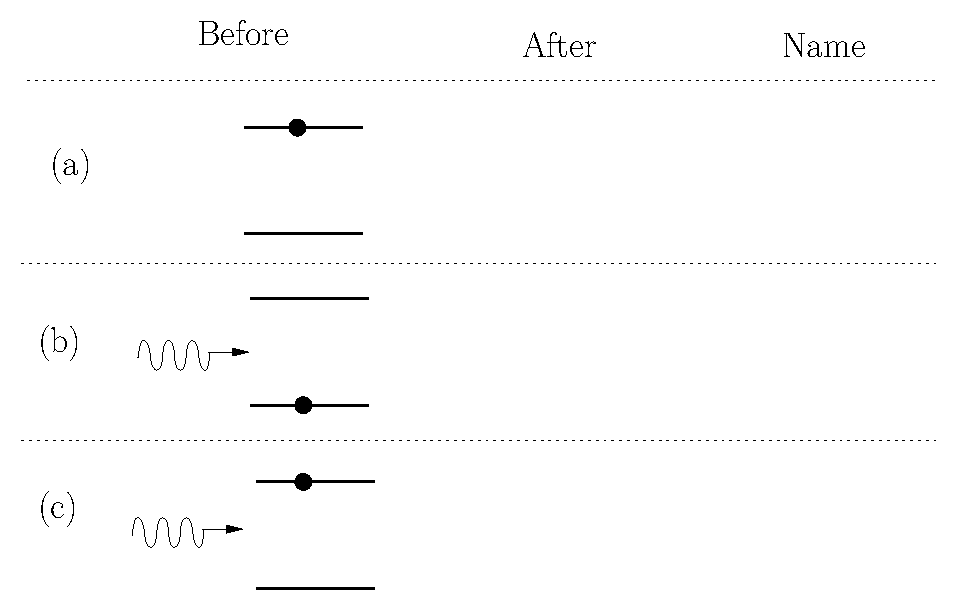
\includegraphics[width=3.5in]{additional_problems/transitions}
      \caption{Problem \ref{prob:transitions}}
      \label{fig:stim_emission}
    \end{center}
  \end{figure}
\end{problem}

\begin{problem}
  {\bf Superconductors.} (Do in Problem Session) Here we investigate
  some magnetic properties of superconductors.

  \begin{enumerate} 
  \item Closely observe the little cube hovering over the disk.
    Comment on what you observe.  What evidence do you have that this
    is a superconductor?  Can you make the cube spin?

  \item Explain how the superconductor can levitate the magnet.

  \end{enumerate}
\end{problem}


\begin{problem}
Why would you not expect helium-3 to act as a superfluid at low
  temperatures, even though helium-4 does?
\label{prob:he3_superfluid}
\end{problem}


\begin{problem}
  Sketch the magnetic field lines outside the north-pole end of a bar
  magnet (the field points generally away from the north pole).  Now,
  using the right-hand rule that relates magnetic field to current,
  sketch the shielding currents that must flow in a flat
  superconducting plate when the north-pole end of the bar magnet is
  held just above the plate.  Pay particular attention to the
  direction of the shielding current.  Does the current in the plate
  repel or attract the bar magnet?
\label{prob:barmagnet}
\end{problem}


\begin{problem} 
  {\em Superconducting magnets.}  One of the most productive uses of
  superconductors is in the fabrication of strong electromagnets
  (e.g., for magnetic resonance imaging in hospitals, or in massive
  particle accelerators).  Consider a superconducting magnet
  constructed from a solenoid of 1000 turns of superconducting wire
  with radius $50\, \mbox{cm}$ and length $1\, \mbox{m}$.  A current
  $I$ is applied, resulting in a magnetic field of 10~Tesla.  Once the
  magnetic field is produced, what power would have to be provided to
  the electromagnet to maintain the magnetic field?
\label{prob:superconducting_magnets}
\end{problem}

%%%%%%%% Hand-Ins %%%%%%%%%%%%%%%%%%%%%%%%%%%%%%%%%%%%%%%%%%%

\begin{problem}
  What would happen if dice were indistinguishable bosons?  Of course,
  real dice are too large for quantum effects to be significant, so
  they are classical, distinguishable objects.  As a result, rolling a
  pair of classical dice yields 36 possible results (1-1, 1-2, 1-3,
  \dots, 6-5, 6-6).
  \begin{enumerate}
  \item Calculate the probability of rolling doubles with real
    (classical) dice.
  \item If dice were indistinguishable bosons, then rolling a 2-5
    combination would be exactly the same as rolling a 5-2
    combination.  How many different results are possible for bosonic
    dice?
  \item How many different ways of rolling doubles are possible with
    bosonic dice?
  \item Use your results from (a) and (b) to calculate the probability
    of rolling doubles with bosonic dice.  Is the probability higher,
    lower, or the same as the classical result?
  \end{enumerate}
\end{problem}



\begin{problem}
  Is it possible to create a quantum state in which one electron in an
  infinite square-well potential is in
  the $n=2$ state with spin up and another
  electron is in the ground state ($n=1$) with
  spin up?  If so, write it out and make sure that it is
  antisymmetric.  If not, explain why not.
\end{problem}


\begin{problem}
  Consider \textit{three} identical particles that are to be put into
  two single-particle states labeled by $|\alpha\rangle$ and
  $|\beta\rangle$.
  \begin{enumerate}
  \item Make three charts like Fig.~\ref{fig:quantum_statistics}
    describing all the possible ways that you can make a
    three-particle state for classical particles, bosons, and
    fermions.  Use the symbols $\bullet$, $\circ$ and $\times$ to
    represent the three distinguishable classical particles, and three
    $\bullet$'s to represent the indistinguishable quantum particles.
  \item How many states are there for the classical particles?  For
    the bosons?  For the fermions?
  \item Assuming that the microstates are equally likely, what is the
    probability of finding the three particles all in the same
    single-particle state for classical particles?  For bosons?
  \item Show how your results are consistent with the idea that bosons have an
    enhanced probability (relative to classical particles) of being in
    the same state, and consistent with the Pauli exclusion principle.
  \end{enumerate}
\end{problem}


\begin{problem}
\label{prob:ruby_laser}
A ruby laser is a solid-state laser that uses a synthetic ruby crystal
as the medium in which stimulated emission occurs as opposed to
individual atoms in a gas laser.  The diagram below shows the energy
levels used in the ruby crystal along with their approximate energies
relative to the ground state.
\begin{enumerate}
\item What is the frequency of the radiation needed to optically pump
  the ruby crystal and therefore create the necessary population
  inversion?
\item What is the wavelength of the emitted laser beam due to
  stimulated emission?
\end{enumerate}

\begin{figure}[h]
\begin{center}
\includegraphics[width=2.4in]{quantum_statistics/ruby_laser}
\caption{Ruby laser energy level diagram for Problem \ref{prob:ruby_laser}}
\label{fig:ruby_laser}
\end{center}
\end{figure}

\end{problem}


\begin{problem}
A superconducting wire of circular cross section has a radius of
$1.5\units{cm}$.  The critical magnetic field that this particular
superconductor can withstand is $B_c=20\units{T}$.  Based on this
information, calculate the maximum current that this superconducting
wire is capable of carrying.  \textit{Hint:} use Ampere's law.
\end{problem}


\begin{problem}
This problem refers to Fig.~\ref{fig:quantum_statistics}, which shows
all the possible ways to put two particles into three states $\ket{\alpha}$,
$\ket{\beta}$, and $\ket{\gamma}$.
\begin{enumerate}
\item For classical particles, take the solid circle to represent
  particle~1 and the open circle to represent particle 2.  Then the
  two-particle state represented in row 4 would be written
  $\ket{\alpha\;\beta}$, while the two-particle state in row 7 would
  be $\ket{\beta\; \alpha}$.  Using this notation, write out 
  the classical two-particle states for each of the nine states given.

\item For  bosons, the two-particle states must be symmetric under
interchange of particles 1 and 2.  Write out the appropriate two-particle
states for each of the six states given.

\item For fermions, the two-particle states must be antisymmetric under
interchange of particles 1 and 2.  Write out the appropriate two-particle
states for each of the three states given.


\end{enumerate}
\end{problem}

%\begin{problem} 
%  {\em Lenz's law (Not) and Superconductors.}  As stated in the
%  reading, if a material in a magnetic field is cooled below its
%  critical temperature $T_c$ for superconductivity, all magnetic
%  fields will be expelled from the interior of the material (the
%  Meissner effect).  This problem shows that Lenz's law cannot be the
%  cause of the Meissner effect, and that superconductors are more than
%  just perfect conductors.
%
%  \begin{enumerate}
%  \item Consider a material with finite conductivity in a magnetic
%    field, as in the left picture of Fig.~\ref{fig:meissner}.  What
%    does Lenz's Law say will happen to the internal magnetic field if
%    the material becomes a perfect conductor (not a superconductor).
%    Contrast this behavior with that of a superconductor.
%  \item Now, assume that the applied magnetic field is turned off.
%    (The material is still a perfect conductor.)  What does Lenz's law
%    say will happen to the internal magnetic field?  Again, contrast
%    this behavior with that of a superconductor.
%  \end{enumerate}
%\label{prob:meissner_and_lenz}
%\end{problem}



%\begin{problem}
%  Superconducting circuit boards.  Several companies have already
%  started making measurement devices with superconducting materials
%  (e.g., extremely fast oscilloscopes).  With high temperature
%  superconductors, cooling these devices is easier than with normal
%  superconductors, since only liquid nitrogen is needed.  Critical
%  currents, however, need to be considered in the design and
%  construction of superconducting circuit boards; specifically,
%  miniaturization can be difficult.  To appreciate this issue, picture
%  a circuit board as being covered with flat traces of conducting
%  materials.  The entire board is cooled below the critical
%  temperature $T_c$ of the traces.
%
%  \begin{enumerate}
%  \item As seen in Problem~\ref{prob:sc_wire}, a limit on the current
%    is provided by critical magnetic fields.  Assuming that the traces
%    must be able to carry $0.1\, \mbox{A}$ of current without losing
%    their superconducting abilities, determine the minimum width of
%    the traces.  Assume a critical field of $1\, \mbox{T}$.  (Hint:
%    approximate this problem as an infinite current sheet, for which
%    the magnetic field is $B = \frac{1}{2}\mu_0\lambda$ near the
%    surface, where $\lambda$ is the current per unit length across the
%    conductor.  Use this result to approximate the relation between
%    the current, the trace width, and the magnetic field strength.)
%  \item Unfortunately, for high temperature superconductors, there is
%    also a critical {\em current density} $J_c \approx 1 \times 10^6\,
%    \mbox{A/m$^2$}$, independent of the critical magnetic field.
%    Assuming the traces to have a thickness of $100\, \mbox{$mu$m}$,
%    estimate the minimum trace width to keep the current density below
%    $J_c$, given a current $I = 0.1\, \mbox{A}$.
%  \end{enumerate}
%  \label{prob:superconducting_circuit_boards}
%\end{problem}

\vfill 

\thispagestyle{empty}
%%%%%%%%%%%%%%%%%%%%%%%%%%%%%%%%%%%%%%%%%%%%%%%%%%%%%%%%%%%%%%%%%%%%%%%%

